%!TEX TS-program = Arara
% arara: pdflatex: {shell: yes}
% arara: biber
% arara: pdflatex: {shell: yes}
\documentclass[12pt,ngerman,DIV=10,
BCOR=1cm,bibliography=totoc,listof=totoc]{scrbook}
\renewcommand*\chapterheadstartvskip{\vspace*{-\topskip}}
%!TEX TS-program = Arara
%!TeX root=Hauptdokument.tex
\usepackage[T1]{fontenc}
\usepackage{booktabs}
\usepackage{babel}
\usepackage{graphicx}
\usepackage{csquotes}
\usepackage{paralist}
\usepackage{xcolor}

\usepackage{prettyref}
% for prettyref
\newrefformat{cha}{Kapitel \ref{#1}}
\newrefformat{sec}{Abschnitt \ref{#1}}
\newrefformat{tab}{Tabelle \ref{#1} auf Seite \pageref{#1}}
\newrefformat{fig}{Bild \ref{#1} auf Seite \pageref{#1}}


\usepackage[style=authoryear-icomp, backend=biber,natbib]{biblatex}
\addbibresource{Literaturverzeichnis.bib}

\usepackage{blindtext}

\usepackage{subcaption}

\usepackage{uni-titlepage}

\author{Zefram Cochrane}
\title{Reisen in Überlichtgeschwindigkeit}
\date{\today}
\place{Köln}
\extratitle{extratitle} % Schmutztitel
\frontispiece{frontispiece} % Bildertitel, https://de.wikipedia.org/wiki/Frontispiz#/media/Datei:Cl%C3%BCver-introductio-1686-1.jpg
\titlehead{Deutsches Zentrum für Luft- und Raumfahrt}
\uppertitleback{uppertitleback}
\lowertitleback{lowertitleback}
\dedication{dedication}
\faculty{Fakultät für Quantenreisen}
\chair{Prof. Dr. Daniel Düsentrieb}
\professor{professor}
\duration{2080--2095}
\referee{Dagobert Duck}
\subject{Dissertation}
%\student{student}
\discipline{discipline}
\matriculationnumber{matriculationnumber}
\advisor{Prof. Dr. Daniel Düsentrieb}
\TitlePageStyle{KIT}

\usepackage{hyperref}
\hypersetup{
    bookmarks=true,                     % show bookmarks bar
    unicode=false,                      % non - Latin characters in Acrobat’s bookmarks
    pdftoolbar=true,                        % show Acrobat’s toolbar
    pdfmenubar=true,                        % show Acrobat’s menu
    pdffitwindow=false,                 % window fit to page when opened
    pdfstartview={FitH},                    % fits the width of the page to the window
    pdftitle={My title},                        % title
    pdfauthor={Author},                 % author
    pdfsubject={Subject},                   % subject of the document
    pdfcreator={Creator},                   % creator of the document
    pdfproducer={Producer},             % producer of the document
    pdfkeywords={keyword1, key2, key3},   % list of keywords
    pdfnewwindow=true,                  % links in new window
    colorlinks=true,                        % false: boxed links; true: colored links
    linkcolor=red,                          % color of internal links
    filecolor=cyan,                     % color of file links
    citecolor=green,                     % color of file links
    urlcolor=magenta                        % color of external links
}



\usepackage[headsepline=0.5pt,footsepline=0.5pt]{scrlayer-scrpage}
\KOMAoptions{headwidth=1.1\textwidth,footwidth=1.1\textwidth}
\pagestyle{scrheadings}
 
\ohead[\headmark]{\headmark}
\ofoot[\pagemark]{\pagemark}
\ifoot[]{\today} % inner foot
\ihead[]{} % inner head
\cfoot[]{} % center foot
\chead[]{} % center head

\newcommand{\pcite}[1]{\citeauthor{#1} (\citeyear{#1})}

\usepackage{chemformula}
\usepackage{mhchem}
\usepackage{siunitx}


\begin{document}
\frontmatter
\maketitle


\tableofcontents

\listoffigures 

\listoftables

\chapter*{Notation}
\addchap{Notation}
%\addcontentsline{toc}{chapter}{Notation}

\mainmatter
%!TeX root=Hauptdokument.tex
\chapter{Einleitung}

Siehe  \prettyref{fig:katze}

\blindtext[3]



In seinem Werk \citetitle{knuth:1984} hat \citeauthor{knuth:1984}, der in Stanford lebt, im Jahr \citeyear{knuth:1984} tolle Dinge beschrieben.

\citetitle{Ziegenhagen2022} von \citeauthor{Ziegenhagen2022}

\cite{ziegenhagen:2017}


\cite{eckstein2022causality}

\blindtext[2]

\blindtext[2]


\blindtext[3]

\ch{CO2}

\prettyref{fig:katze}

\SI{123}{\celsius}



\citep{knuth:1984}

\clearpage

\citet{knuth:1984}


%!TeX root=Hauptdokument.tex
\chapter{Physikalische Grundlagen}

\section{Literatur -- Von Asimoov bis Kirk}

\blindtext[3]

\begin{center}
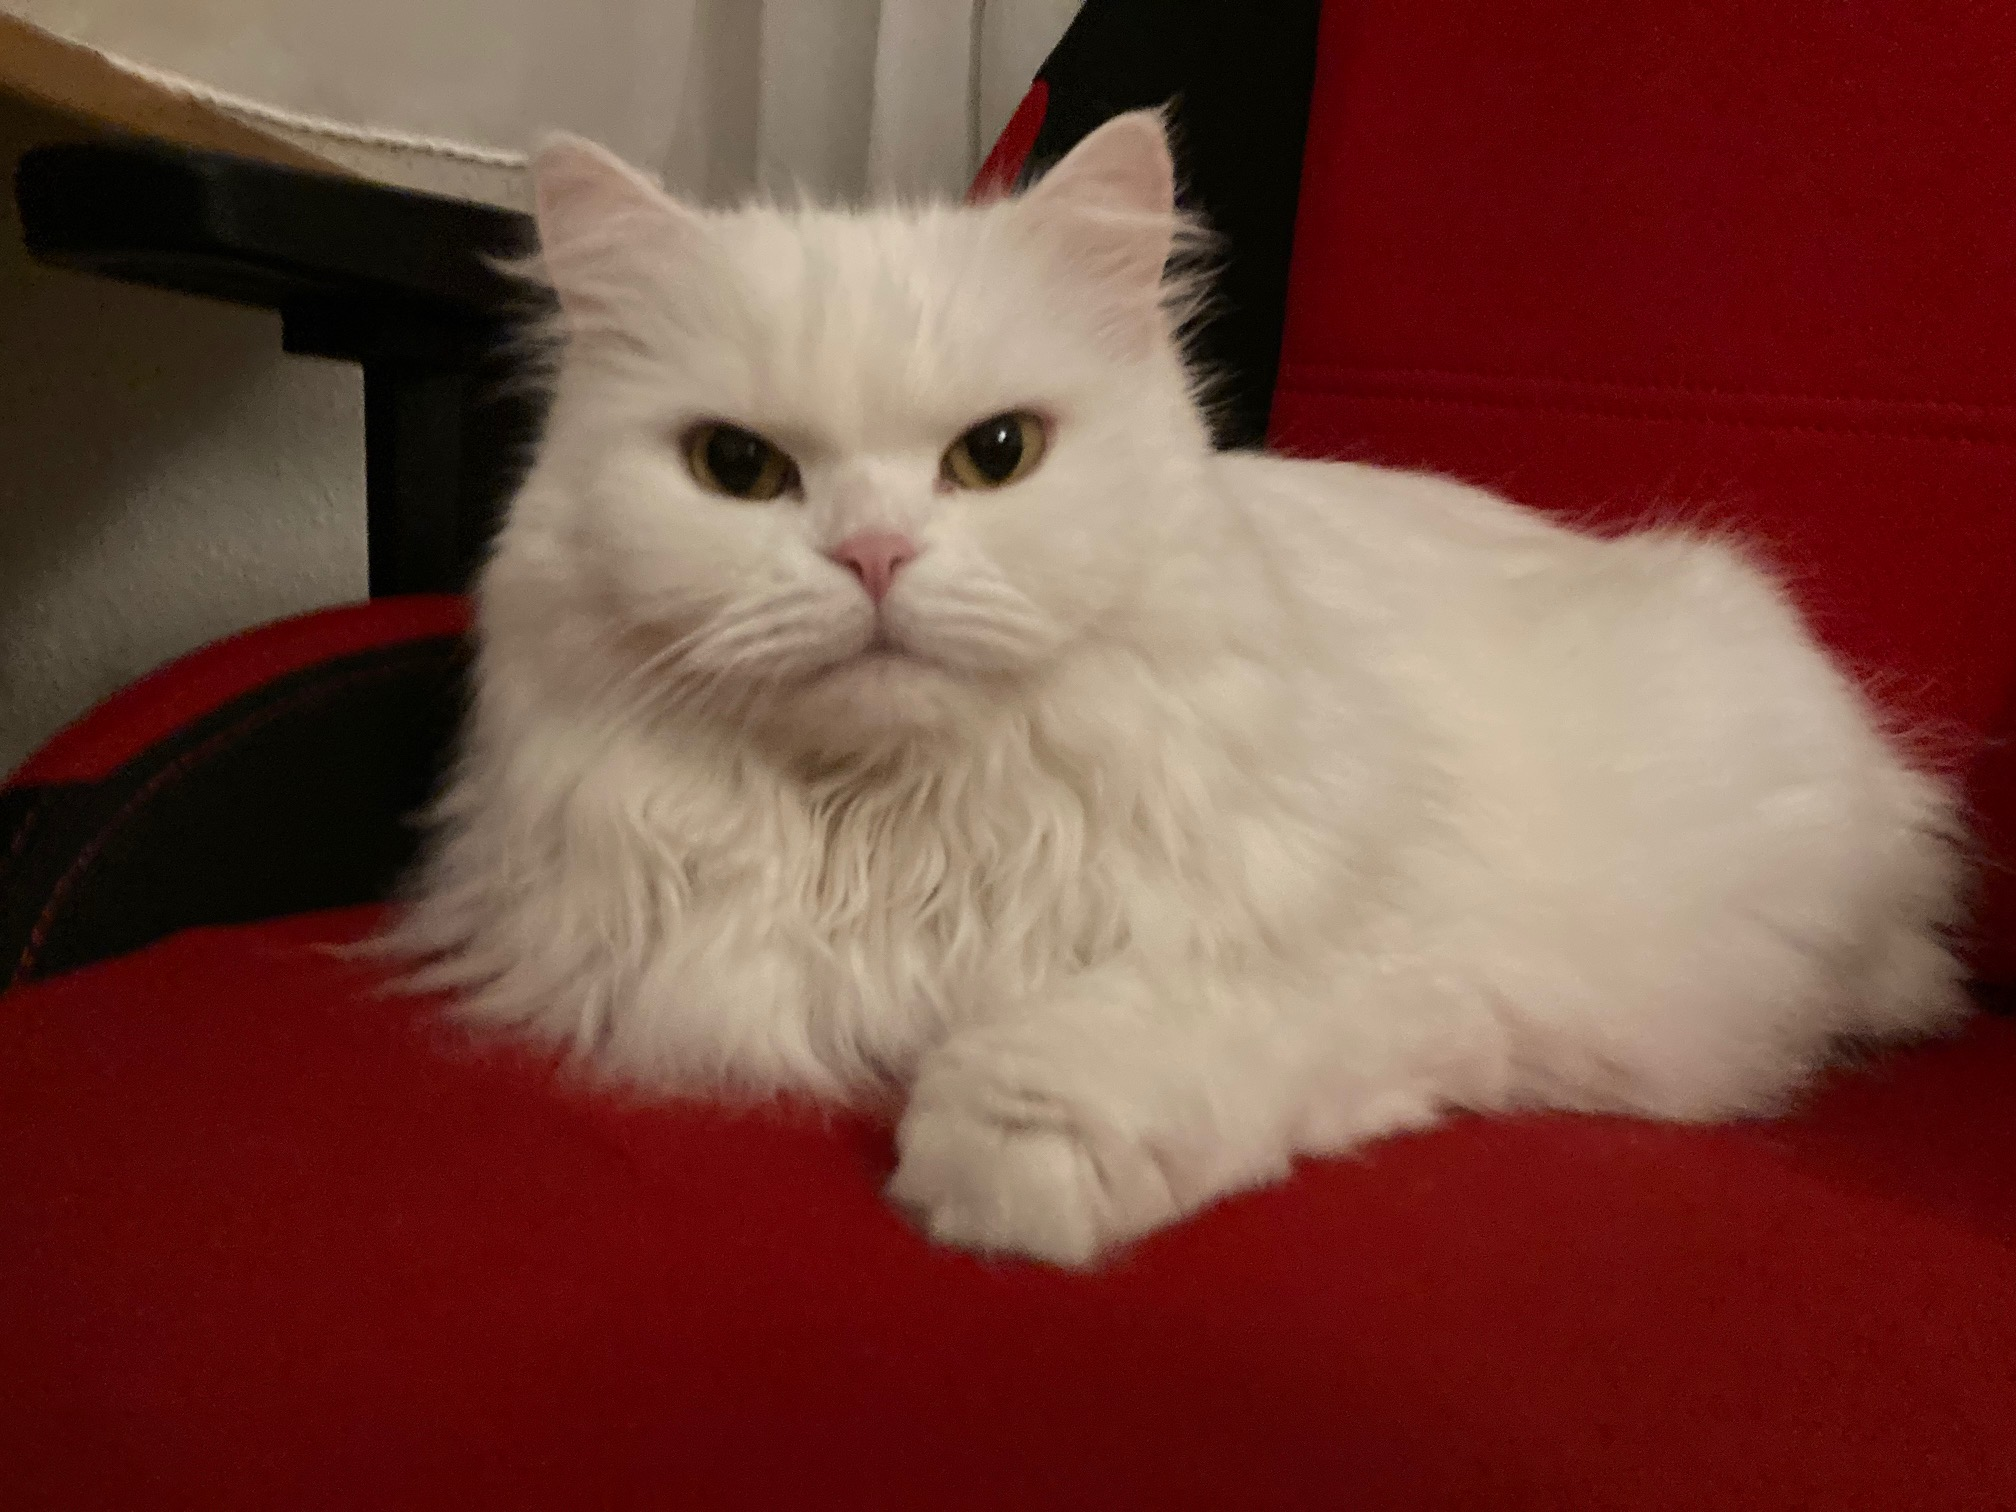
\includegraphics[width=0.8\textwidth]{Bilder/Katze.jpg}
\captionof{figure}{Meine Katze Melli}\label{fig:katze}
\end{center}


\blindtext[3]

\begin{figure}
\centering
\subcaptionbox{Eine Katze \label{cat1}}
{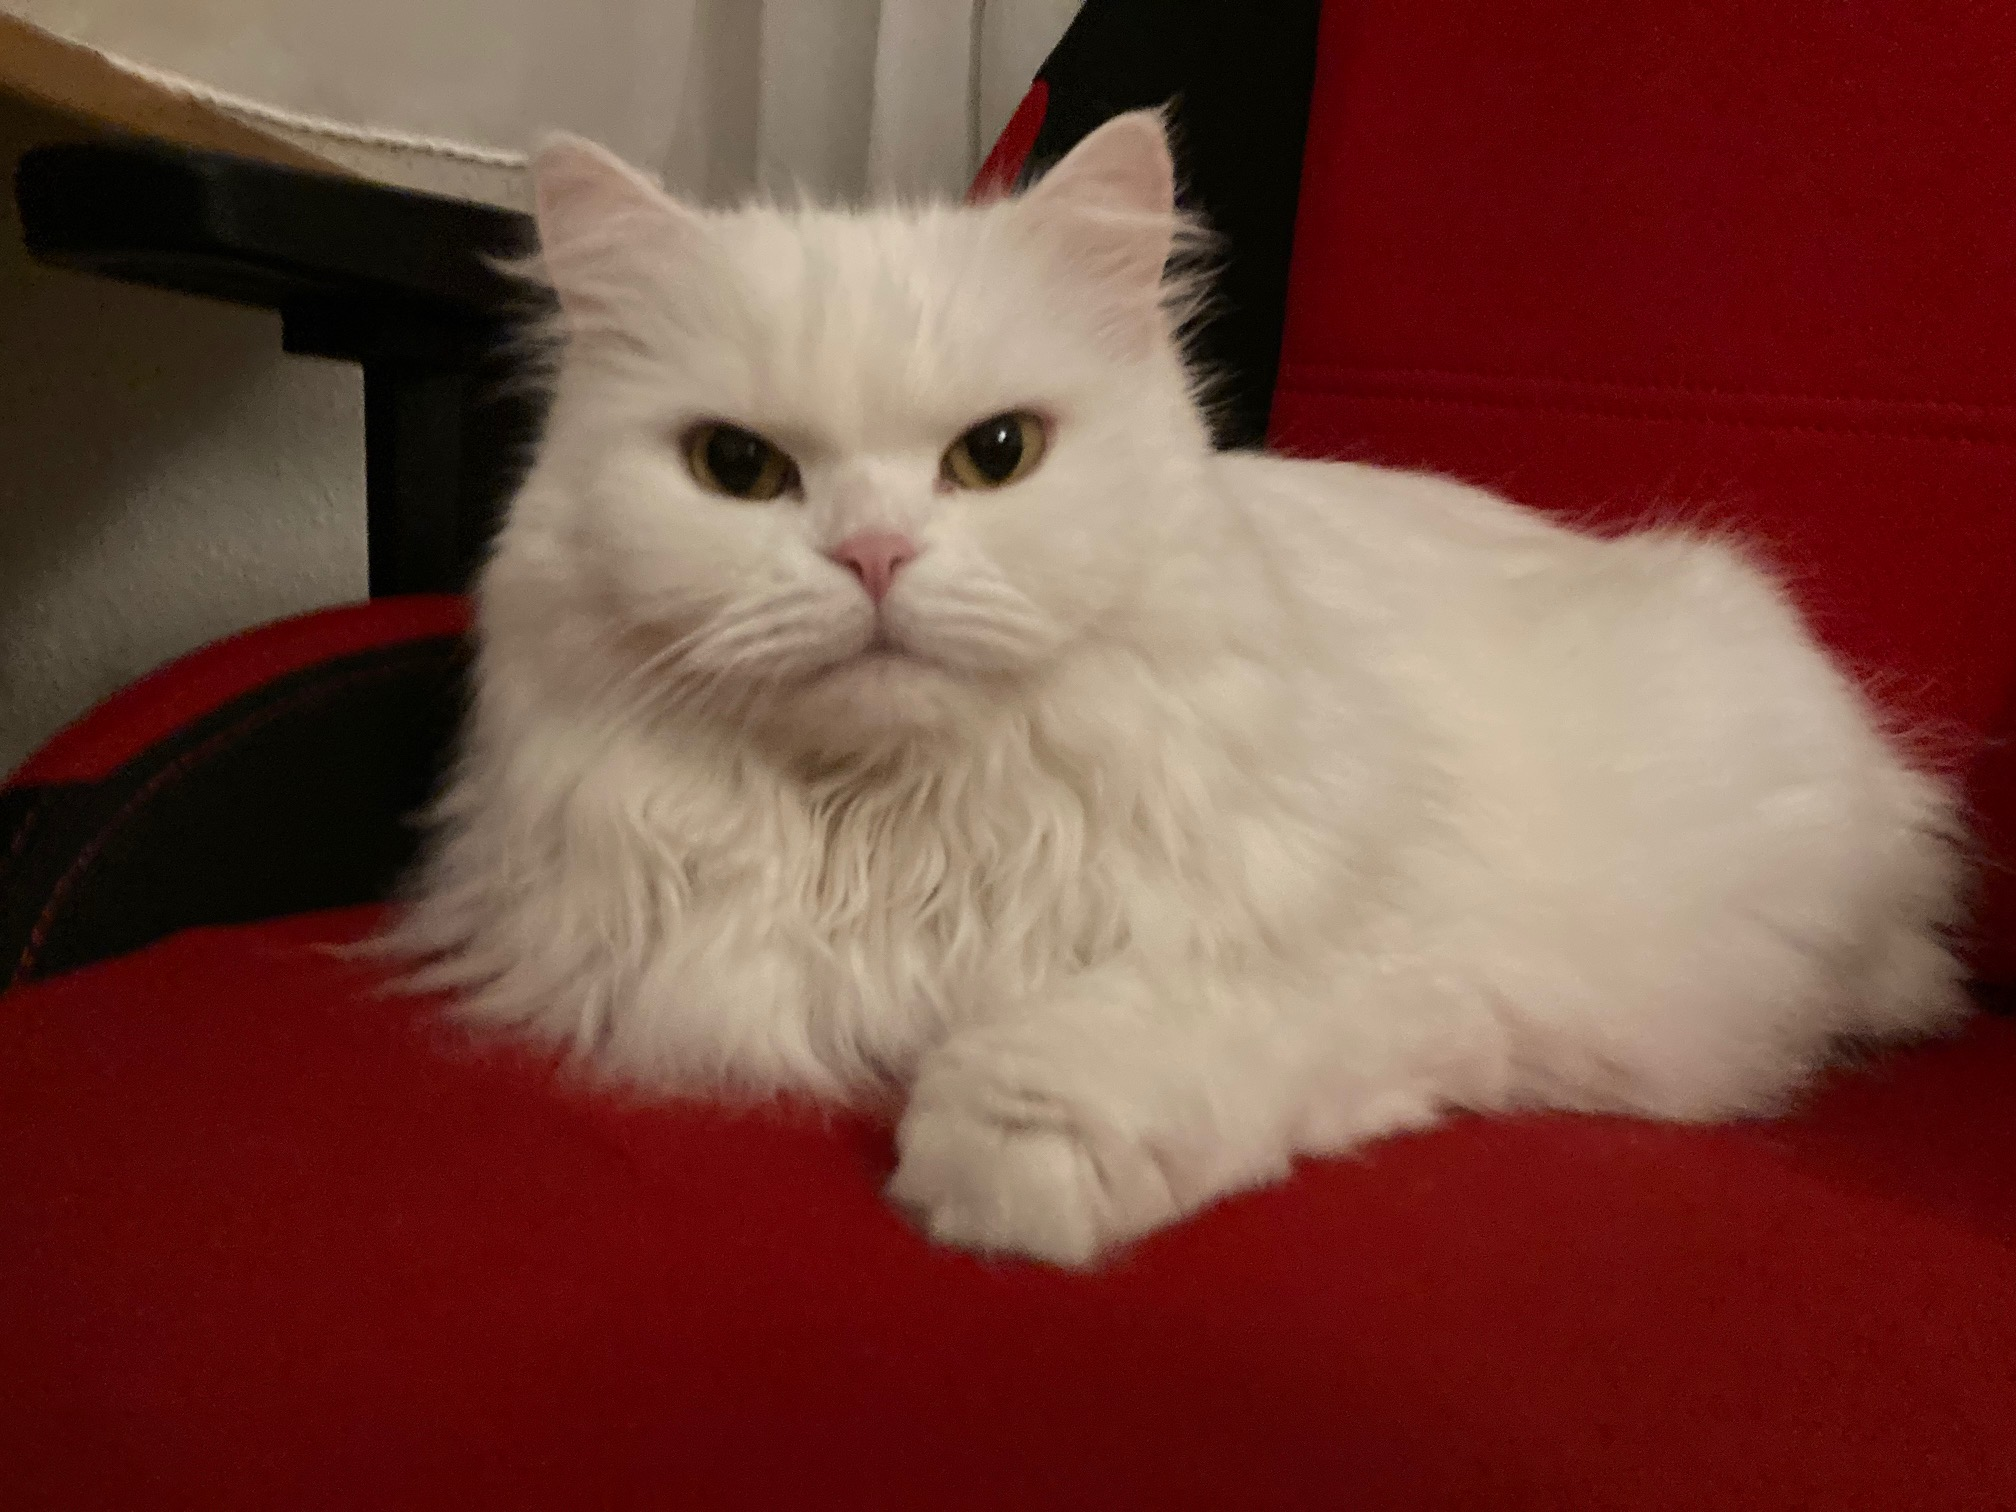
\includegraphics[width=0.49\textwidth]{Bilder/Katze}}
\subcaptionbox{Die selbe Katze \label{cat2}}
{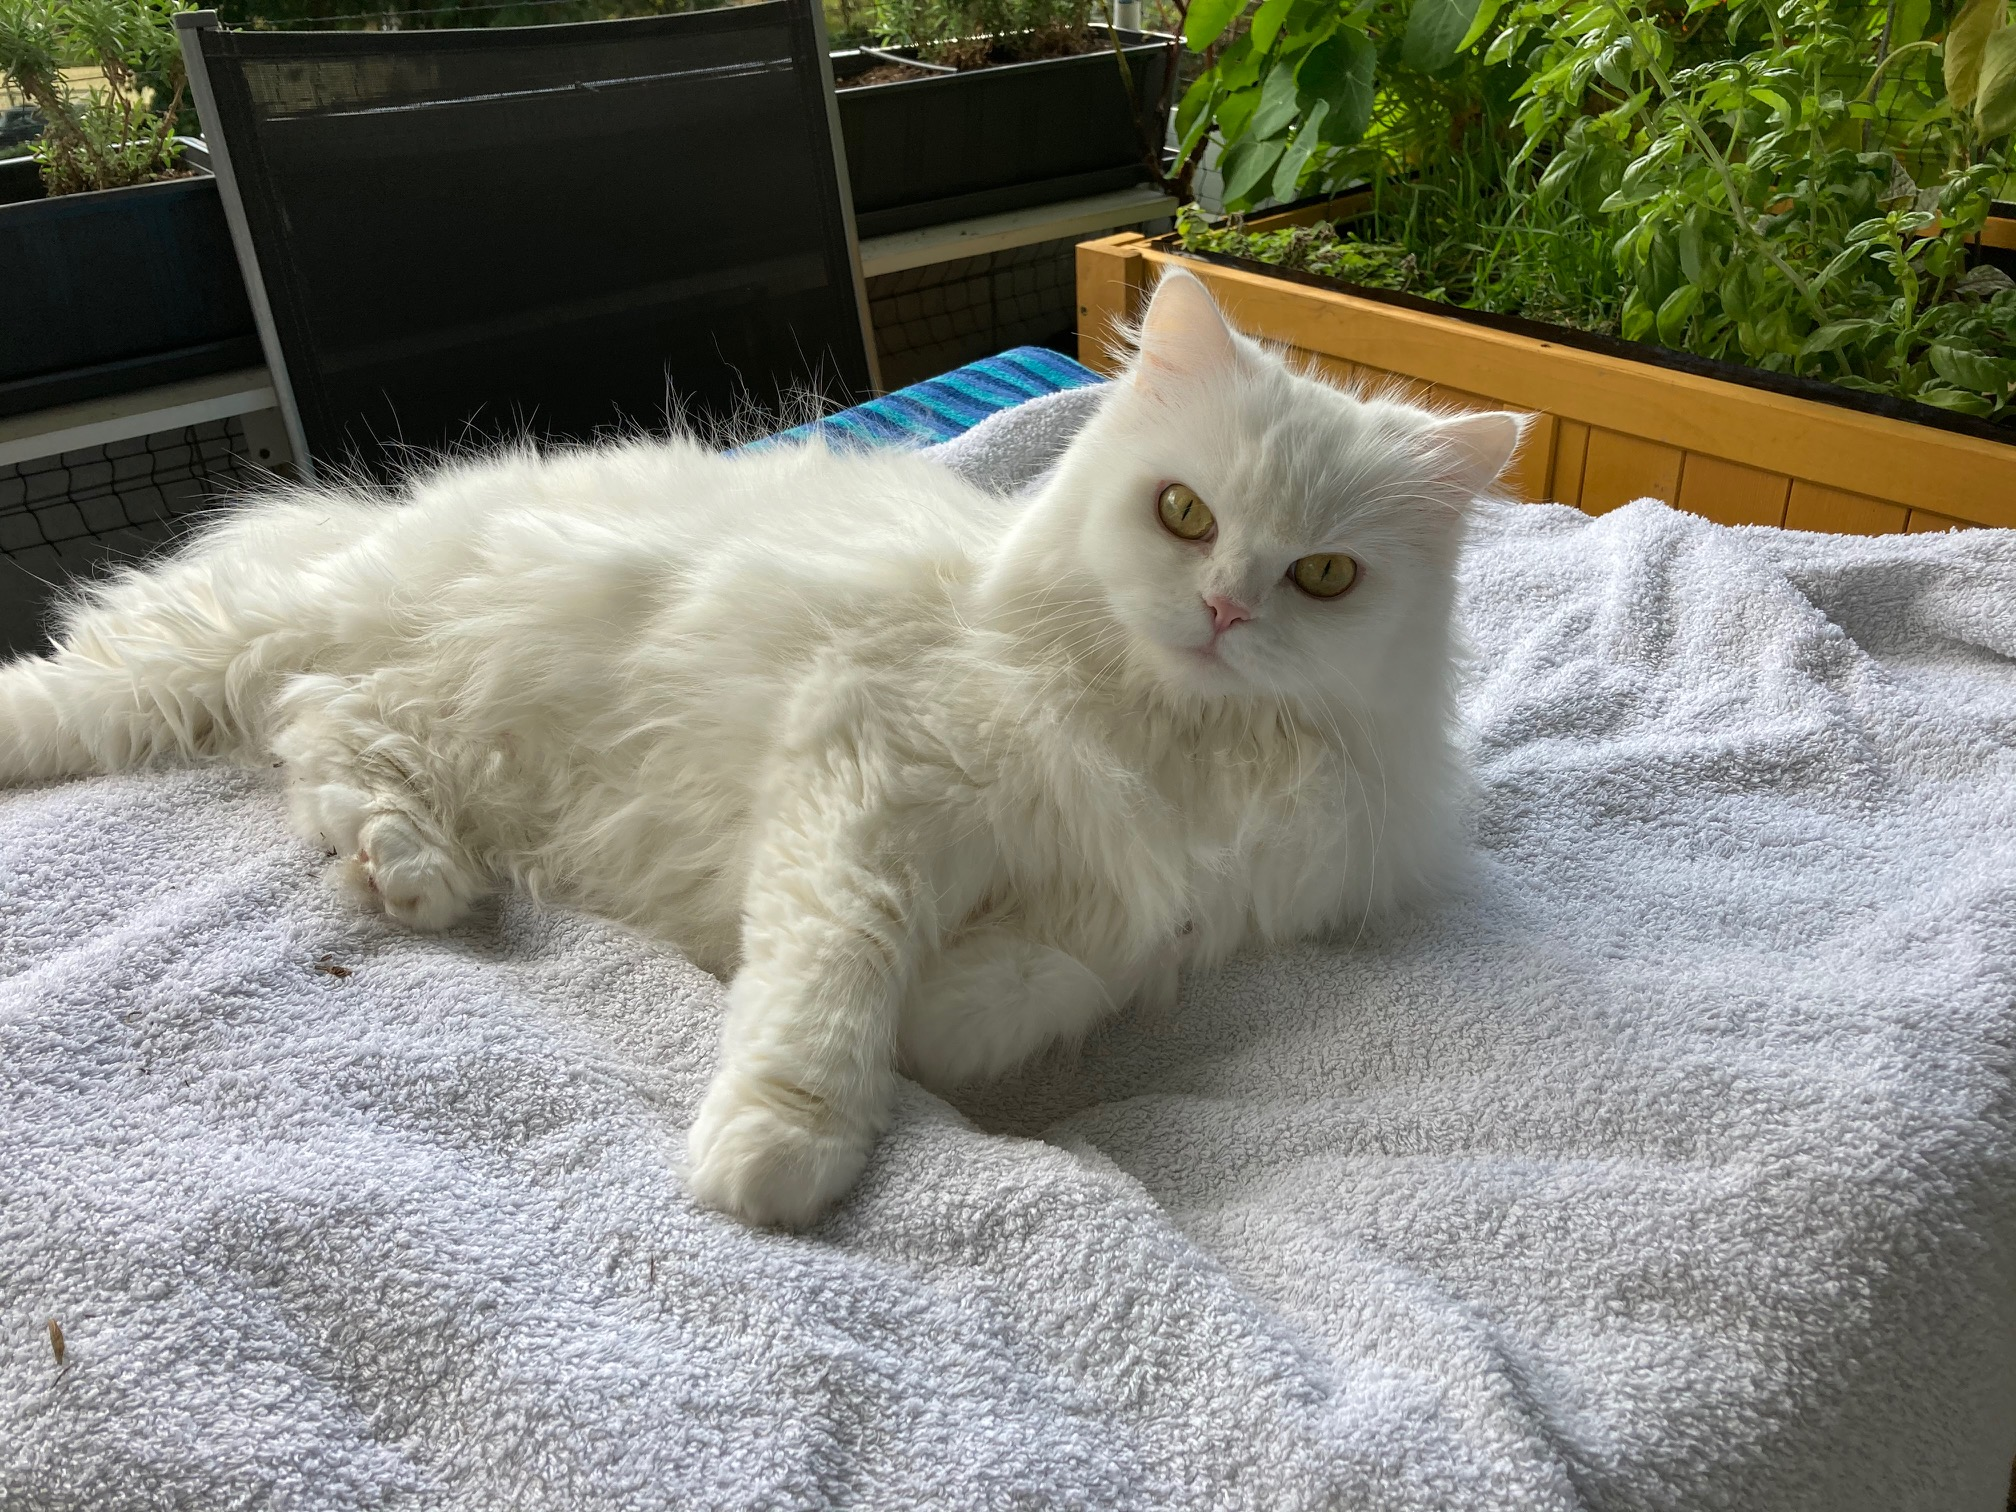
\includegraphics[width=0.49\textwidth]{Bilder/Katze1}}
%\caption{Zwei Katzenbilder}\label{katzenbilder}
\subcaptionbox{Eine Katze \label{cat1}}
{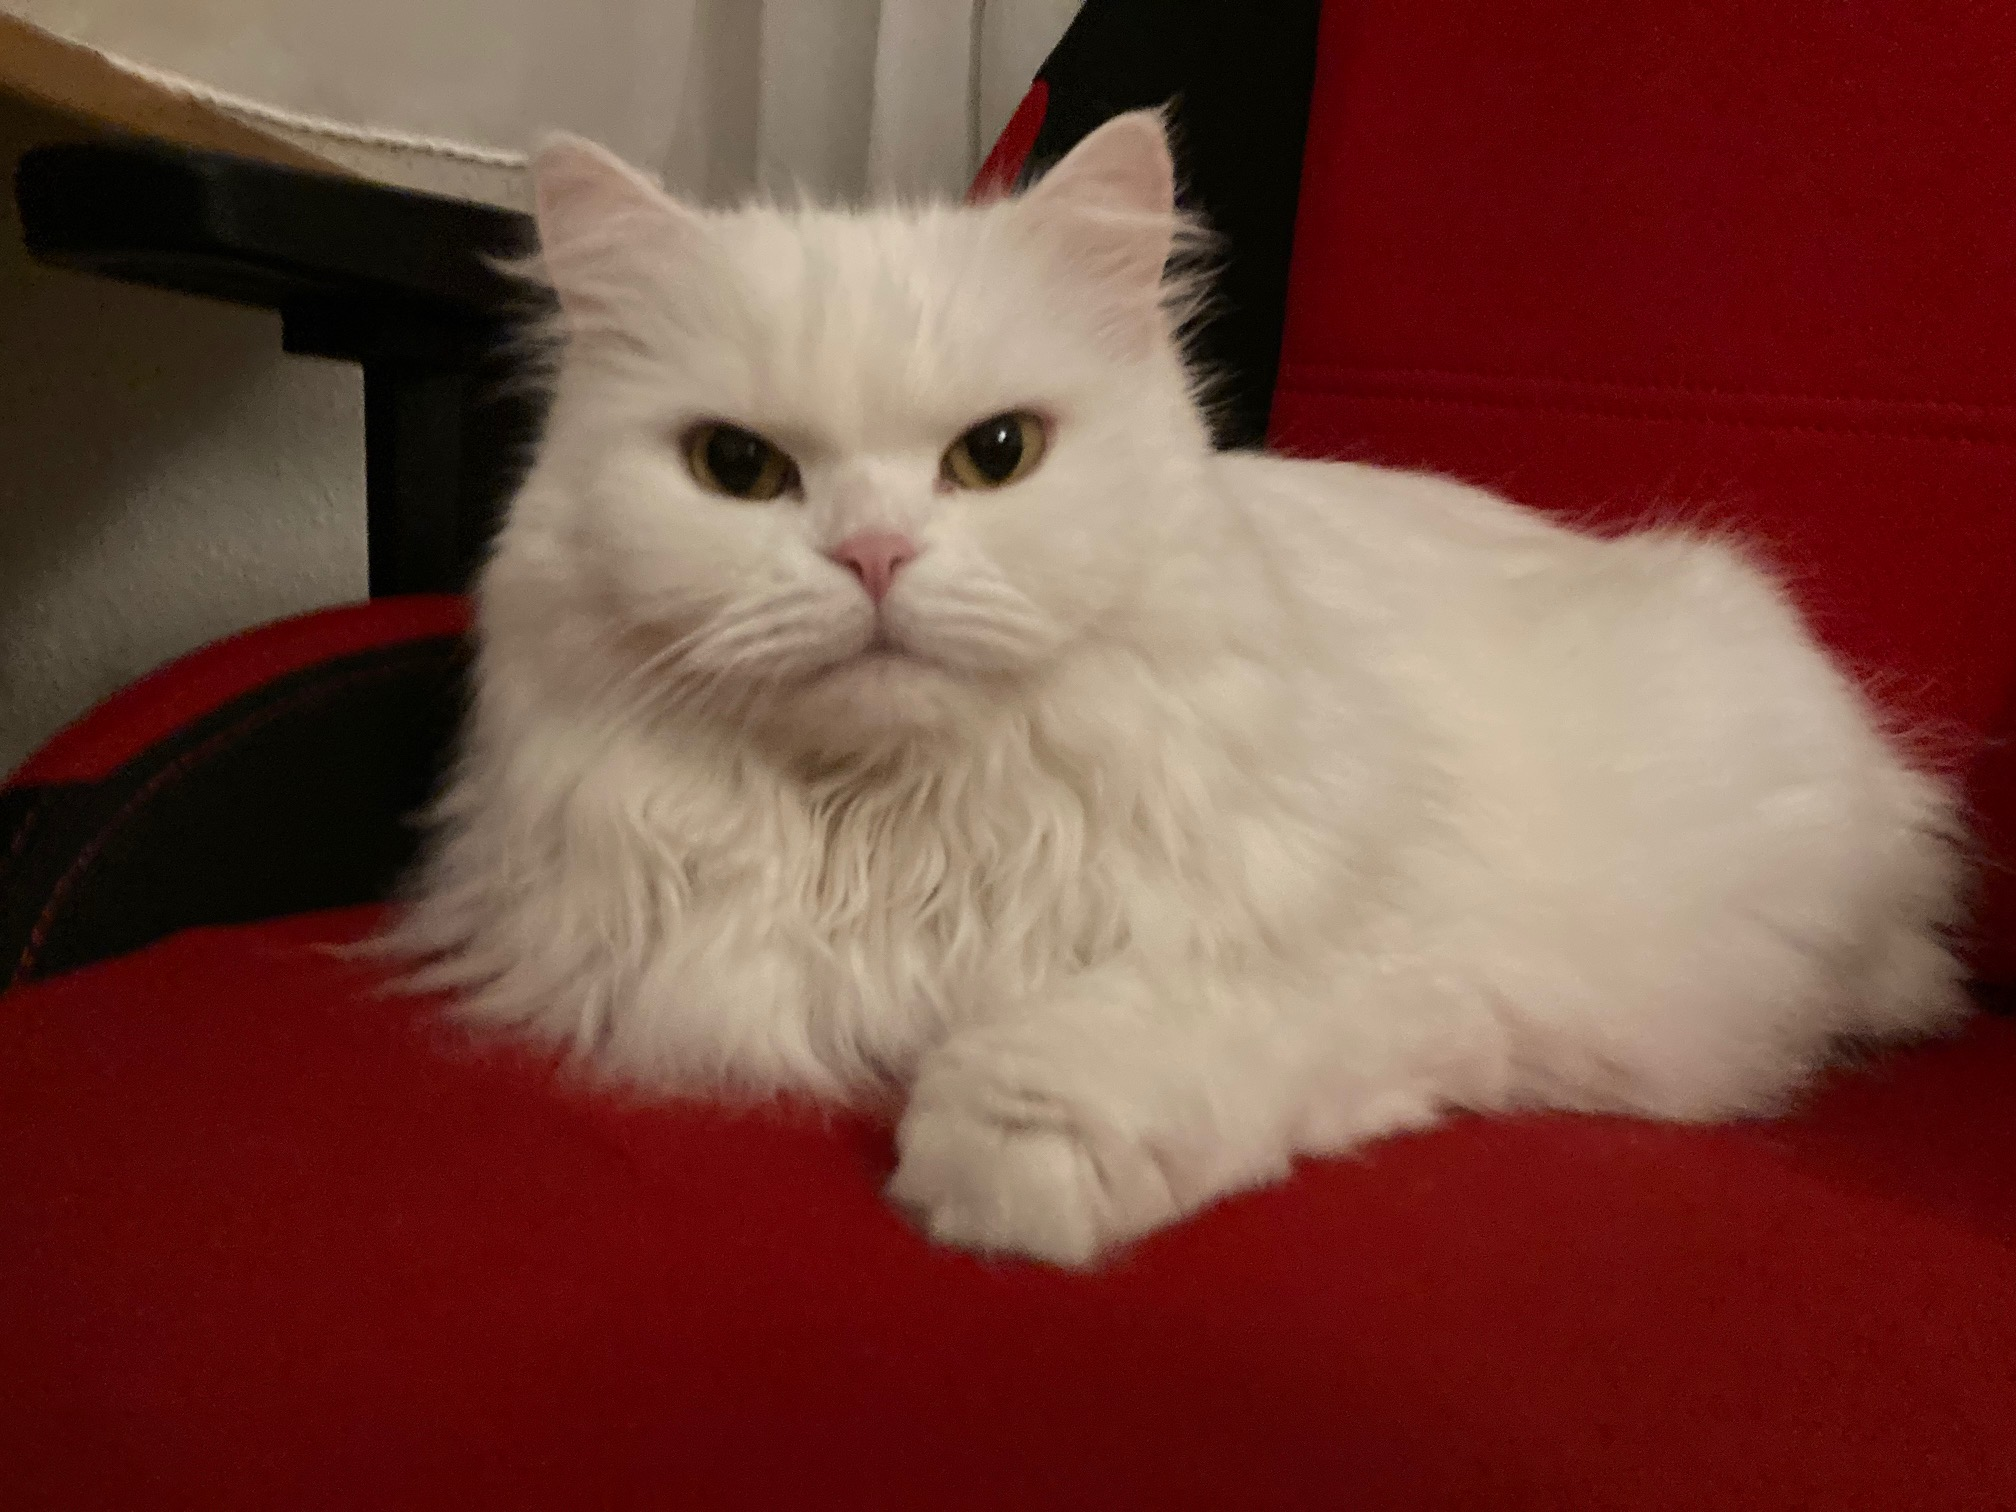
\includegraphics[width=0.49\textwidth]{Bilder/Katze}}
\subcaptionbox{Die selbe Katze \label{cat2}}
{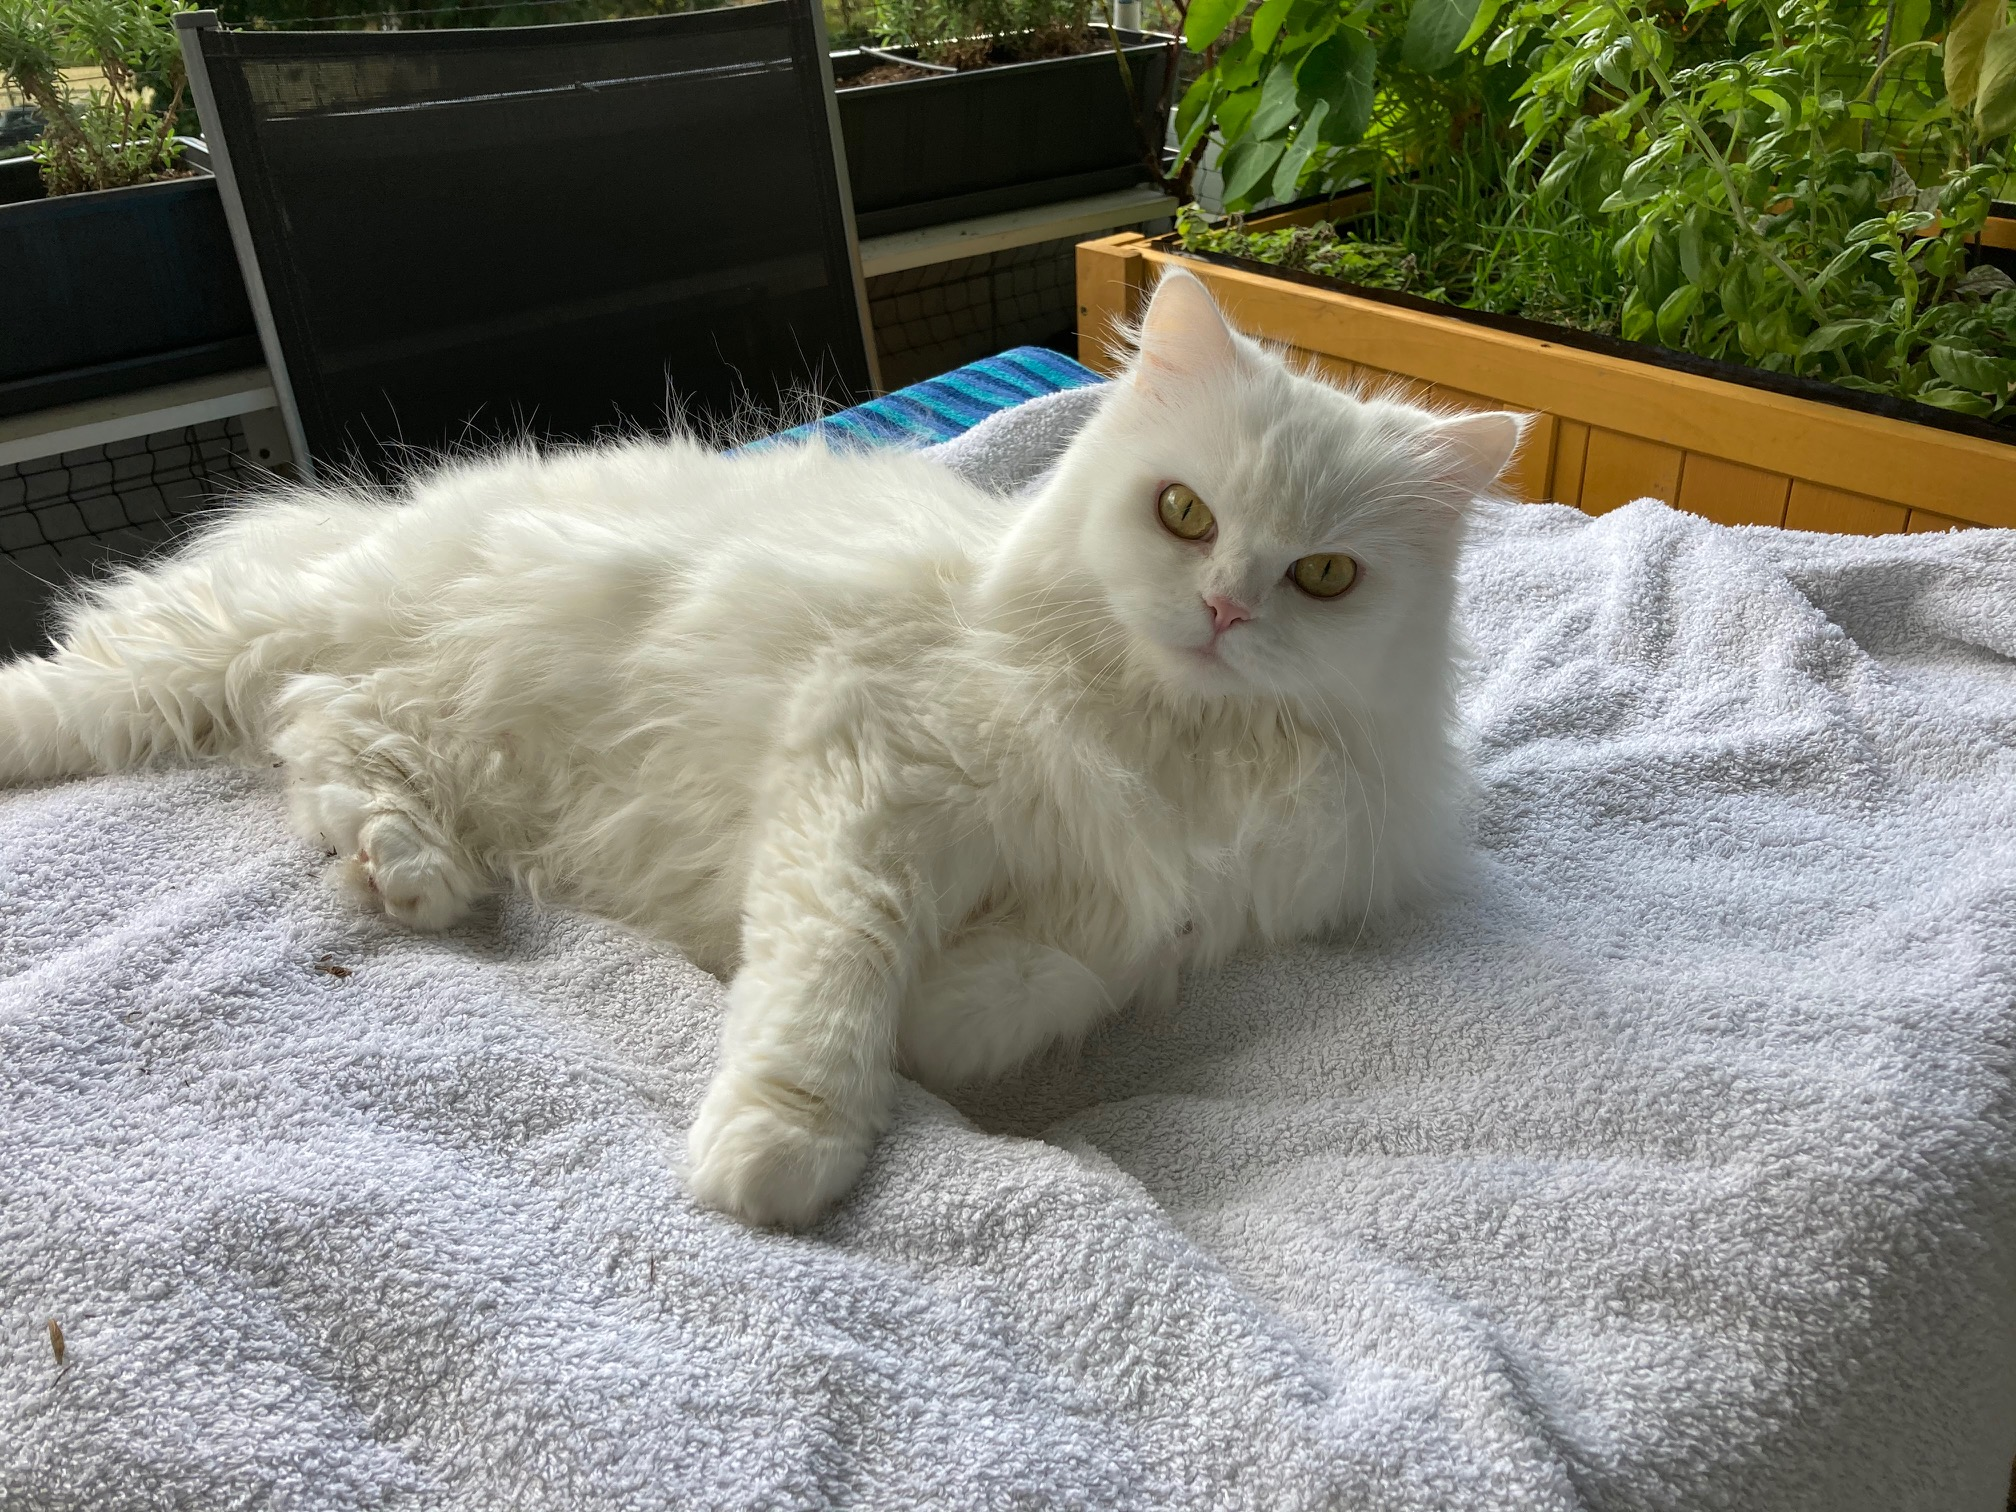
\includegraphics[width=0.49\textwidth]{Bilder/Katze1}}
\caption{Zwei Katzenbilder}\label{katzenbilder}
\end{figure}

Abbildung \ref{cat1} auf Seite \pageref{katzenbilder}

Abbildung \ref{cat2} auf Seite \pageref{katzenbilder}

Abbildung \ref{katzenbilder} auf Seite \pageref{katzenbilder}



\blindtext[3]

\blindtext[3]

\backmatter
\printbibliography

\end{document}